% Created by tikzDevice version 0.10.1 on 2017-11-07 14:46:40
% !TEX encoding = UTF-8 Unicode
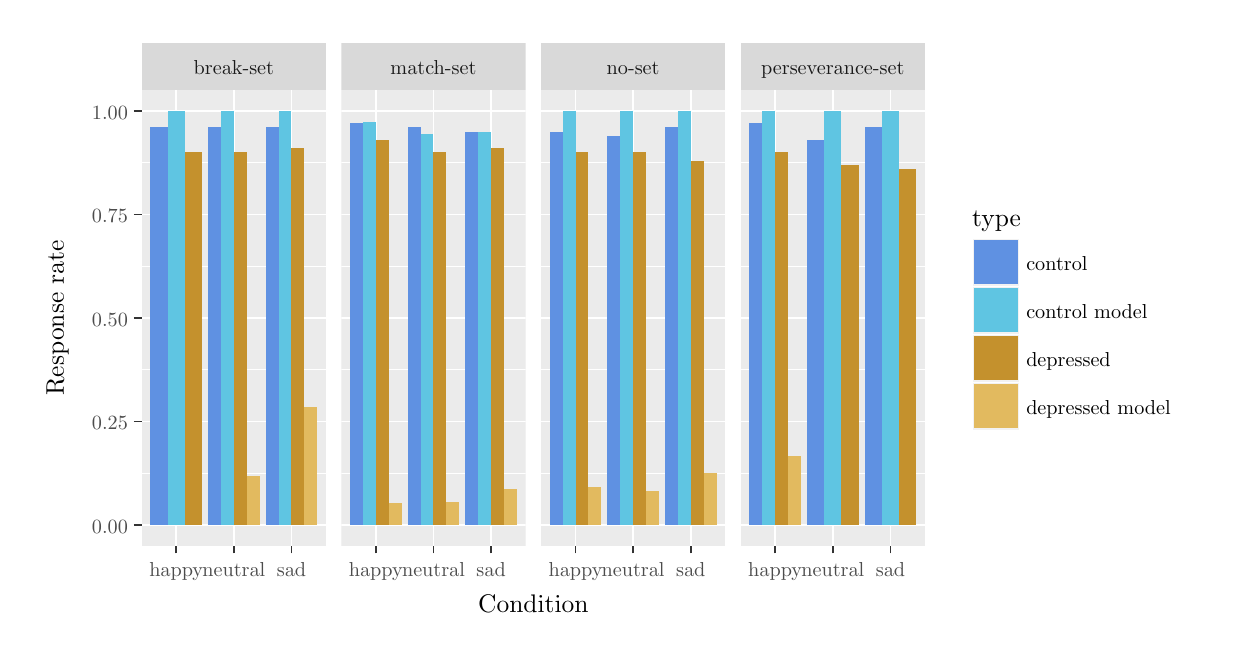
\begin{tikzpicture}[x=1pt,y=1pt]
\definecolor{fillColor}{RGB}{255,255,255}
\path[use as bounding box,fill=fillColor,fill opacity=0.00] (0,0) rectangle (433.62,216.81);
\begin{scope}
\path[clip] (  0.00,  0.00) rectangle (433.62,216.81);
\definecolor{drawColor}{RGB}{255,255,255}
\definecolor{fillColor}{RGB}{255,255,255}

\path[draw=drawColor,line width= 0.6pt,line join=round,line cap=round,fill=fillColor] (  0.00,  0.00) rectangle (433.62,216.81);
\end{scope}
\begin{scope}
\path[clip] ( 41.17, 29.59) rectangle (107.82,194.25);
\definecolor{fillColor}{gray}{0.92}

\path[fill=fillColor] ( 41.17, 29.59) rectangle (107.82,194.25);
\definecolor{drawColor}{RGB}{255,255,255}

\path[draw=drawColor,line width= 0.3pt,line join=round] ( 41.17, 55.78) --
	(107.82, 55.78);

\path[draw=drawColor,line width= 0.3pt,line join=round] ( 41.17, 93.21) --
	(107.82, 93.21);

\path[draw=drawColor,line width= 0.3pt,line join=round] ( 41.17,130.63) --
	(107.82,130.63);

\path[draw=drawColor,line width= 0.3pt,line join=round] ( 41.17,168.05) --
	(107.82,168.05);

\path[draw=drawColor,line width= 0.6pt,line join=round] ( 41.17, 37.07) --
	(107.82, 37.07);

\path[draw=drawColor,line width= 0.6pt,line join=round] ( 41.17, 74.49) --
	(107.82, 74.49);

\path[draw=drawColor,line width= 0.6pt,line join=round] ( 41.17,111.92) --
	(107.82,111.92);

\path[draw=drawColor,line width= 0.6pt,line join=round] ( 41.17,149.34) --
	(107.82,149.34);

\path[draw=drawColor,line width= 0.6pt,line join=round] ( 41.17,186.76) --
	(107.82,186.76);

\path[draw=drawColor,line width= 0.6pt,line join=round] ( 53.67, 29.59) --
	( 53.67,194.25);

\path[draw=drawColor,line width= 0.6pt,line join=round] ( 74.50, 29.59) --
	( 74.50,194.25);

\path[draw=drawColor,line width= 0.6pt,line join=round] ( 95.32, 29.59) --
	( 95.32,194.25);
\definecolor{fillColor}{RGB}{196,145,45}

\path[fill=fillColor] ( 56.79, 37.07) rectangle ( 63.04,171.80);
\definecolor{fillColor}{RGB}{95,197,226}

\path[fill=fillColor] ( 50.55, 37.07) rectangle ( 56.79,186.76);
\definecolor{fillColor}{RGB}{95,145,226}

\path[fill=fillColor] ( 44.30, 37.07) rectangle ( 50.55,180.78);
\definecolor{fillColor}{RGB}{226,186,95}

\path[fill=fillColor] ( 79.18, 37.07) rectangle ( 83.87, 54.68);
\definecolor{fillColor}{RGB}{196,145,45}

\path[fill=fillColor] ( 74.50, 37.07) rectangle ( 79.18,171.80);
\definecolor{fillColor}{RGB}{95,197,226}

\path[fill=fillColor] ( 69.81, 37.07) rectangle ( 74.50,186.76);
\definecolor{fillColor}{RGB}{95,145,226}

\path[fill=fillColor] ( 65.12, 37.07) rectangle ( 69.81,180.78);
\definecolor{fillColor}{RGB}{226,186,95}

\path[fill=fillColor] (100.01, 37.07) rectangle (104.69, 79.84);
\definecolor{fillColor}{RGB}{196,145,45}

\path[fill=fillColor] ( 95.32, 37.07) rectangle (100.01,173.29);
\definecolor{fillColor}{RGB}{95,197,226}

\path[fill=fillColor] ( 90.64, 37.07) rectangle ( 95.32,186.76);
\definecolor{fillColor}{RGB}{95,145,226}

\path[fill=fillColor] ( 85.95, 37.07) rectangle ( 90.64,180.78);
\end{scope}
\begin{scope}
\path[clip] (113.32, 29.59) rectangle (179.96,194.25);
\definecolor{fillColor}{gray}{0.92}

\path[fill=fillColor] (113.32, 29.59) rectangle (179.96,194.25);
\definecolor{drawColor}{RGB}{255,255,255}

\path[draw=drawColor,line width= 0.3pt,line join=round] (113.32, 55.78) --
	(179.96, 55.78);

\path[draw=drawColor,line width= 0.3pt,line join=round] (113.32, 93.21) --
	(179.96, 93.21);

\path[draw=drawColor,line width= 0.3pt,line join=round] (113.32,130.63) --
	(179.96,130.63);

\path[draw=drawColor,line width= 0.3pt,line join=round] (113.32,168.05) --
	(179.96,168.05);

\path[draw=drawColor,line width= 0.6pt,line join=round] (113.32, 37.07) --
	(179.96, 37.07);

\path[draw=drawColor,line width= 0.6pt,line join=round] (113.32, 74.49) --
	(179.96, 74.49);

\path[draw=drawColor,line width= 0.6pt,line join=round] (113.32,111.92) --
	(179.96,111.92);

\path[draw=drawColor,line width= 0.6pt,line join=round] (113.32,149.34) --
	(179.96,149.34);

\path[draw=drawColor,line width= 0.6pt,line join=round] (113.32,186.76) --
	(179.96,186.76);

\path[draw=drawColor,line width= 0.6pt,line join=round] (125.81, 29.59) --
	(125.81,194.25);

\path[draw=drawColor,line width= 0.6pt,line join=round] (146.64, 29.59) --
	(146.64,194.25);

\path[draw=drawColor,line width= 0.6pt,line join=round] (167.47, 29.59) --
	(167.47,194.25);
\definecolor{fillColor}{RGB}{226,186,95}

\path[fill=fillColor] (130.50, 37.07) rectangle (135.19, 45.16);
\definecolor{fillColor}{RGB}{196,145,45}

\path[fill=fillColor] (125.81, 37.07) rectangle (130.50,176.29);
\definecolor{fillColor}{RGB}{95,197,226}

\path[fill=fillColor] (121.13, 37.07) rectangle (125.81,182.61);
\definecolor{fillColor}{RGB}{95,145,226}

\path[fill=fillColor] (116.44, 37.07) rectangle (121.13,182.27);
\definecolor{fillColor}{RGB}{226,186,95}

\path[fill=fillColor] (151.33, 37.07) rectangle (156.01, 45.39);
\definecolor{fillColor}{RGB}{196,145,45}

\path[fill=fillColor] (146.64, 37.07) rectangle (151.33,171.80);
\definecolor{fillColor}{RGB}{95,197,226}

\path[fill=fillColor] (141.95, 37.07) rectangle (146.64,178.21);
\definecolor{fillColor}{RGB}{95,145,226}

\path[fill=fillColor] (137.27, 37.07) rectangle (141.95,180.78);
\definecolor{fillColor}{RGB}{226,186,95}

\path[fill=fillColor] (172.15, 37.07) rectangle (176.84, 50.09);
\definecolor{fillColor}{RGB}{196,145,45}

\path[fill=fillColor] (167.47, 37.07) rectangle (172.15,173.29);
\definecolor{fillColor}{RGB}{95,197,226}

\path[fill=fillColor] (162.78, 37.07) rectangle (167.47,179.09);
\definecolor{fillColor}{RGB}{95,145,226}

\path[fill=fillColor] (158.10, 37.07) rectangle (162.78,179.28);
\end{scope}
\begin{scope}
\path[clip] (185.46, 29.59) rectangle (252.11,194.25);
\definecolor{fillColor}{gray}{0.92}

\path[fill=fillColor] (185.46, 29.59) rectangle (252.11,194.25);
\definecolor{drawColor}{RGB}{255,255,255}

\path[draw=drawColor,line width= 0.3pt,line join=round] (185.46, 55.78) --
	(252.11, 55.78);

\path[draw=drawColor,line width= 0.3pt,line join=round] (185.46, 93.21) --
	(252.11, 93.21);

\path[draw=drawColor,line width= 0.3pt,line join=round] (185.46,130.63) --
	(252.11,130.63);

\path[draw=drawColor,line width= 0.3pt,line join=round] (185.46,168.05) --
	(252.11,168.05);

\path[draw=drawColor,line width= 0.6pt,line join=round] (185.46, 37.07) --
	(252.11, 37.07);

\path[draw=drawColor,line width= 0.6pt,line join=round] (185.46, 74.49) --
	(252.11, 74.49);

\path[draw=drawColor,line width= 0.6pt,line join=round] (185.46,111.92) --
	(252.11,111.92);

\path[draw=drawColor,line width= 0.6pt,line join=round] (185.46,149.34) --
	(252.11,149.34);

\path[draw=drawColor,line width= 0.6pt,line join=round] (185.46,186.76) --
	(252.11,186.76);

\path[draw=drawColor,line width= 0.6pt,line join=round] (197.96, 29.59) --
	(197.96,194.25);

\path[draw=drawColor,line width= 0.6pt,line join=round] (218.79, 29.59) --
	(218.79,194.25);

\path[draw=drawColor,line width= 0.6pt,line join=round] (239.61, 29.59) --
	(239.61,194.25);
\definecolor{fillColor}{RGB}{226,186,95}

\path[fill=fillColor] (202.64, 37.07) rectangle (207.33, 51.00);
\definecolor{fillColor}{RGB}{196,145,45}

\path[fill=fillColor] (197.96, 37.07) rectangle (202.64,171.80);
\definecolor{fillColor}{RGB}{95,197,226}

\path[fill=fillColor] (193.27, 37.07) rectangle (197.96,186.76);
\definecolor{fillColor}{RGB}{95,145,226}

\path[fill=fillColor] (188.59, 37.07) rectangle (193.27,179.28);
\definecolor{fillColor}{RGB}{226,186,95}

\path[fill=fillColor] (223.47, 37.07) rectangle (228.16, 49.29);
\definecolor{fillColor}{RGB}{196,145,45}

\path[fill=fillColor] (218.79, 37.07) rectangle (223.47,171.80);
\definecolor{fillColor}{RGB}{95,197,226}

\path[fill=fillColor] (214.10, 37.07) rectangle (218.79,186.76);
\definecolor{fillColor}{RGB}{95,145,226}

\path[fill=fillColor] (209.41, 37.07) rectangle (214.10,177.78);
\definecolor{fillColor}{RGB}{226,186,95}

\path[fill=fillColor] (244.30, 37.07) rectangle (248.98, 55.78);
\definecolor{fillColor}{RGB}{196,145,45}

\path[fill=fillColor] (239.61, 37.07) rectangle (244.30,168.80);
\definecolor{fillColor}{RGB}{95,197,226}

\path[fill=fillColor] (234.93, 37.07) rectangle (239.61,186.76);
\definecolor{fillColor}{RGB}{95,145,226}

\path[fill=fillColor] (230.24, 37.07) rectangle (234.93,180.78);
\end{scope}
\begin{scope}
\path[clip] (257.61, 29.59) rectangle (324.25,194.25);
\definecolor{fillColor}{gray}{0.92}

\path[fill=fillColor] (257.61, 29.59) rectangle (324.25,194.25);
\definecolor{drawColor}{RGB}{255,255,255}

\path[draw=drawColor,line width= 0.3pt,line join=round] (257.61, 55.78) --
	(324.25, 55.78);

\path[draw=drawColor,line width= 0.3pt,line join=round] (257.61, 93.21) --
	(324.25, 93.21);

\path[draw=drawColor,line width= 0.3pt,line join=round] (257.61,130.63) --
	(324.25,130.63);

\path[draw=drawColor,line width= 0.3pt,line join=round] (257.61,168.05) --
	(324.25,168.05);

\path[draw=drawColor,line width= 0.6pt,line join=round] (257.61, 37.07) --
	(324.25, 37.07);

\path[draw=drawColor,line width= 0.6pt,line join=round] (257.61, 74.49) --
	(324.25, 74.49);

\path[draw=drawColor,line width= 0.6pt,line join=round] (257.61,111.92) --
	(324.25,111.92);

\path[draw=drawColor,line width= 0.6pt,line join=round] (257.61,149.34) --
	(324.25,149.34);

\path[draw=drawColor,line width= 0.6pt,line join=round] (257.61,186.76) --
	(324.25,186.76);

\path[draw=drawColor,line width= 0.6pt,line join=round] (270.10, 29.59) --
	(270.10,194.25);

\path[draw=drawColor,line width= 0.6pt,line join=round] (290.93, 29.59) --
	(290.93,194.25);

\path[draw=drawColor,line width= 0.6pt,line join=round] (311.76, 29.59) --
	(311.76,194.25);
\definecolor{fillColor}{RGB}{226,186,95}

\path[fill=fillColor] (274.79, 37.07) rectangle (279.48, 62.02);
\definecolor{fillColor}{RGB}{196,145,45}

\path[fill=fillColor] (270.10, 37.07) rectangle (274.79,171.80);
\definecolor{fillColor}{RGB}{95,197,226}

\path[fill=fillColor] (265.42, 37.07) rectangle (270.10,186.76);
\definecolor{fillColor}{RGB}{95,145,226}

\path[fill=fillColor] (260.73, 37.07) rectangle (265.42,182.27);
\definecolor{fillColor}{RGB}{196,145,45}

\path[fill=fillColor] (294.05, 37.07) rectangle (300.30,167.30);
\definecolor{fillColor}{RGB}{95,197,226}

\path[fill=fillColor] (287.81, 37.07) rectangle (294.05,186.76);
\definecolor{fillColor}{RGB}{95,145,226}

\path[fill=fillColor] (281.56, 37.07) rectangle (287.81,176.29);
\definecolor{fillColor}{RGB}{196,145,45}

\path[fill=fillColor] (314.88, 37.07) rectangle (321.13,165.81);
\definecolor{fillColor}{RGB}{95,197,226}

\path[fill=fillColor] (308.63, 37.07) rectangle (314.88,186.76);
\definecolor{fillColor}{RGB}{95,145,226}

\path[fill=fillColor] (302.39, 37.07) rectangle (308.63,180.78);
\end{scope}
\begin{scope}
\path[clip] ( 41.17,194.25) rectangle (107.82,211.31);
\definecolor{fillColor}{gray}{0.85}

\path[fill=fillColor] ( 41.17,194.25) rectangle (107.82,211.31);
\definecolor{drawColor}{gray}{0.10}

\node[text=drawColor,anchor=base,inner sep=0pt, outer sep=0pt, scale=  0.73] at ( 74.50,199.75) {break-set};
\end{scope}
\begin{scope}
\path[clip] (113.32,194.25) rectangle (179.96,211.31);
\definecolor{fillColor}{gray}{0.85}

\path[fill=fillColor] (113.32,194.25) rectangle (179.96,211.31);
\definecolor{drawColor}{gray}{0.10}

\node[text=drawColor,anchor=base,inner sep=0pt, outer sep=0pt, scale=  0.73] at (146.64,199.75) {match-set};
\end{scope}
\begin{scope}
\path[clip] (185.46,194.25) rectangle (252.11,211.31);
\definecolor{fillColor}{gray}{0.85}

\path[fill=fillColor] (185.46,194.25) rectangle (252.11,211.31);
\definecolor{drawColor}{gray}{0.10}

\node[text=drawColor,anchor=base,inner sep=0pt, outer sep=0pt, scale=  0.73] at (218.79,199.75) {no-set};
\end{scope}
\begin{scope}
\path[clip] (257.61,194.25) rectangle (324.25,211.31);
\definecolor{fillColor}{gray}{0.85}

\path[fill=fillColor] (257.61,194.25) rectangle (324.25,211.31);
\definecolor{drawColor}{gray}{0.10}

\node[text=drawColor,anchor=base,inner sep=0pt, outer sep=0pt, scale=  0.73] at (290.93,199.75) {perseverance-set};
\end{scope}
\begin{scope}
\path[clip] (  0.00,  0.00) rectangle (433.62,216.81);
\definecolor{drawColor}{gray}{0.20}

\path[draw=drawColor,line width= 0.6pt,line join=round] ( 53.67, 26.84) --
	( 53.67, 29.59);

\path[draw=drawColor,line width= 0.6pt,line join=round] ( 74.50, 26.84) --
	( 74.50, 29.59);

\path[draw=drawColor,line width= 0.6pt,line join=round] ( 95.32, 26.84) --
	( 95.32, 29.59);
\end{scope}
\begin{scope}
\path[clip] (  0.00,  0.00) rectangle (433.62,216.81);
\definecolor{drawColor}{gray}{0.30}

\node[text=drawColor,anchor=base,inner sep=0pt, outer sep=0pt, scale=  0.73] at ( 53.67, 18.58) {happy};

\node[text=drawColor,anchor=base,inner sep=0pt, outer sep=0pt, scale=  0.73] at ( 74.50, 18.58) {neutral};

\node[text=drawColor,anchor=base,inner sep=0pt, outer sep=0pt, scale=  0.73] at ( 95.32, 18.58) {sad};
\end{scope}
\begin{scope}
\path[clip] (  0.00,  0.00) rectangle (433.62,216.81);
\definecolor{drawColor}{gray}{0.20}

\path[draw=drawColor,line width= 0.6pt,line join=round] (125.81, 26.84) --
	(125.81, 29.59);

\path[draw=drawColor,line width= 0.6pt,line join=round] (146.64, 26.84) --
	(146.64, 29.59);

\path[draw=drawColor,line width= 0.6pt,line join=round] (167.47, 26.84) --
	(167.47, 29.59);
\end{scope}
\begin{scope}
\path[clip] (  0.00,  0.00) rectangle (433.62,216.81);
\definecolor{drawColor}{gray}{0.30}

\node[text=drawColor,anchor=base,inner sep=0pt, outer sep=0pt, scale=  0.73] at (125.81, 18.58) {happy};

\node[text=drawColor,anchor=base,inner sep=0pt, outer sep=0pt, scale=  0.73] at (146.64, 18.58) {neutral};

\node[text=drawColor,anchor=base,inner sep=0pt, outer sep=0pt, scale=  0.73] at (167.47, 18.58) {sad};
\end{scope}
\begin{scope}
\path[clip] (  0.00,  0.00) rectangle (433.62,216.81);
\definecolor{drawColor}{gray}{0.20}

\path[draw=drawColor,line width= 0.6pt,line join=round] (197.96, 26.84) --
	(197.96, 29.59);

\path[draw=drawColor,line width= 0.6pt,line join=round] (218.79, 26.84) --
	(218.79, 29.59);

\path[draw=drawColor,line width= 0.6pt,line join=round] (239.61, 26.84) --
	(239.61, 29.59);
\end{scope}
\begin{scope}
\path[clip] (  0.00,  0.00) rectangle (433.62,216.81);
\definecolor{drawColor}{gray}{0.30}

\node[text=drawColor,anchor=base,inner sep=0pt, outer sep=0pt, scale=  0.73] at (197.96, 18.58) {happy};

\node[text=drawColor,anchor=base,inner sep=0pt, outer sep=0pt, scale=  0.73] at (218.79, 18.58) {neutral};

\node[text=drawColor,anchor=base,inner sep=0pt, outer sep=0pt, scale=  0.73] at (239.61, 18.58) {sad};
\end{scope}
\begin{scope}
\path[clip] (  0.00,  0.00) rectangle (433.62,216.81);
\definecolor{drawColor}{gray}{0.20}

\path[draw=drawColor,line width= 0.6pt,line join=round] (270.10, 26.84) --
	(270.10, 29.59);

\path[draw=drawColor,line width= 0.6pt,line join=round] (290.93, 26.84) --
	(290.93, 29.59);

\path[draw=drawColor,line width= 0.6pt,line join=round] (311.76, 26.84) --
	(311.76, 29.59);
\end{scope}
\begin{scope}
\path[clip] (  0.00,  0.00) rectangle (433.62,216.81);
\definecolor{drawColor}{gray}{0.30}

\node[text=drawColor,anchor=base,inner sep=0pt, outer sep=0pt, scale=  0.73] at (270.10, 18.58) {happy};

\node[text=drawColor,anchor=base,inner sep=0pt, outer sep=0pt, scale=  0.73] at (290.93, 18.58) {neutral};

\node[text=drawColor,anchor=base,inner sep=0pt, outer sep=0pt, scale=  0.73] at (311.76, 18.58) {sad};
\end{scope}
\begin{scope}
\path[clip] (  0.00,  0.00) rectangle (433.62,216.81);
\definecolor{drawColor}{gray}{0.30}

\node[text=drawColor,anchor=base east,inner sep=0pt, outer sep=0pt, scale=  0.73] at ( 36.22, 34.04) {0.00};

\node[text=drawColor,anchor=base east,inner sep=0pt, outer sep=0pt, scale=  0.73] at ( 36.22, 71.46) {0.25};

\node[text=drawColor,anchor=base east,inner sep=0pt, outer sep=0pt, scale=  0.73] at ( 36.22,108.89) {0.50};

\node[text=drawColor,anchor=base east,inner sep=0pt, outer sep=0pt, scale=  0.73] at ( 36.22,146.31) {0.75};

\node[text=drawColor,anchor=base east,inner sep=0pt, outer sep=0pt, scale=  0.73] at ( 36.22,183.73) {1.00};
\end{scope}
\begin{scope}
\path[clip] (  0.00,  0.00) rectangle (433.62,216.81);
\definecolor{drawColor}{gray}{0.20}

\path[draw=drawColor,line width= 0.6pt,line join=round] ( 38.42, 37.07) --
	( 41.17, 37.07);

\path[draw=drawColor,line width= 0.6pt,line join=round] ( 38.42, 74.49) --
	( 41.17, 74.49);

\path[draw=drawColor,line width= 0.6pt,line join=round] ( 38.42,111.92) --
	( 41.17,111.92);

\path[draw=drawColor,line width= 0.6pt,line join=round] ( 38.42,149.34) --
	( 41.17,149.34);

\path[draw=drawColor,line width= 0.6pt,line join=round] ( 38.42,186.76) --
	( 41.17,186.76);
\end{scope}
\begin{scope}
\path[clip] (  0.00,  0.00) rectangle (433.62,216.81);
\definecolor{drawColor}{RGB}{0,0,0}

\node[text=drawColor,anchor=base,inner sep=0pt, outer sep=0pt, scale=  0.92] at (182.71,  5.50) {Condition};
\end{scope}
\begin{scope}
\path[clip] (  0.00,  0.00) rectangle (433.62,216.81);
\definecolor{drawColor}{RGB}{0,0,0}

\node[text=drawColor,rotate= 90.00,anchor=base,inner sep=0pt, outer sep=0pt, scale=  0.92] at ( 13.08,111.92) {Response rate};
\end{scope}
\begin{scope}
\path[clip] (  0.00,  0.00) rectangle (433.62,216.81);
\definecolor{fillColor}{RGB}{255,255,255}

\path[fill=fillColor] (335.63, 65.58) rectangle (428.12,158.25);
\end{scope}
\begin{scope}
\path[clip] (  0.00,  0.00) rectangle (433.62,216.81);
\definecolor{drawColor}{RGB}{0,0,0}

\node[text=drawColor,anchor=base west,inner sep=0pt, outer sep=0pt, scale=  0.92] at (341.32,144.99) {type};
\end{scope}
\begin{scope}
\path[clip] (  0.00,  0.00) rectangle (433.62,216.81);
\definecolor{drawColor}{RGB}{255,255,255}
\definecolor{fillColor}{gray}{0.95}

\path[draw=drawColor,line width= 0.6pt,line join=round,line cap=round,fill=fillColor] (341.32,123.31) rectangle (358.67,140.65);
\end{scope}
\begin{scope}
\path[clip] (  0.00,  0.00) rectangle (433.62,216.81);
\definecolor{fillColor}{RGB}{95,145,226}

\path[fill=fillColor] (342.04,124.02) rectangle (357.96,139.94);
\end{scope}
\begin{scope}
\path[clip] (  0.00,  0.00) rectangle (433.62,216.81);
\definecolor{drawColor}{RGB}{255,255,255}
\definecolor{fillColor}{gray}{0.95}

\path[draw=drawColor,line width= 0.6pt,line join=round,line cap=round,fill=fillColor] (341.32,105.96) rectangle (358.67,123.31);
\end{scope}
\begin{scope}
\path[clip] (  0.00,  0.00) rectangle (433.62,216.81);
\definecolor{fillColor}{RGB}{95,197,226}

\path[fill=fillColor] (342.04,106.67) rectangle (357.96,122.60);
\end{scope}
\begin{scope}
\path[clip] (  0.00,  0.00) rectangle (433.62,216.81);
\definecolor{drawColor}{RGB}{255,255,255}
\definecolor{fillColor}{gray}{0.95}

\path[draw=drawColor,line width= 0.6pt,line join=round,line cap=round,fill=fillColor] (341.32, 88.62) rectangle (358.67,105.96);
\end{scope}
\begin{scope}
\path[clip] (  0.00,  0.00) rectangle (433.62,216.81);
\definecolor{fillColor}{RGB}{196,145,45}

\path[fill=fillColor] (342.04, 89.33) rectangle (357.96,105.25);
\end{scope}
\begin{scope}
\path[clip] (  0.00,  0.00) rectangle (433.62,216.81);
\definecolor{drawColor}{RGB}{255,255,255}
\definecolor{fillColor}{gray}{0.95}

\path[draw=drawColor,line width= 0.6pt,line join=round,line cap=round,fill=fillColor] (341.32, 71.27) rectangle (358.67, 88.62);
\end{scope}
\begin{scope}
\path[clip] (  0.00,  0.00) rectangle (433.62,216.81);
\definecolor{fillColor}{RGB}{226,186,95}

\path[fill=fillColor] (342.04, 71.98) rectangle (357.96, 87.91);
\end{scope}
\begin{scope}
\path[clip] (  0.00,  0.00) rectangle (433.62,216.81);
\definecolor{drawColor}{RGB}{0,0,0}

\node[text=drawColor,anchor=base west,inner sep=0pt, outer sep=0pt, scale=  0.73] at (360.84,128.95) {control};
\end{scope}
\begin{scope}
\path[clip] (  0.00,  0.00) rectangle (433.62,216.81);
\definecolor{drawColor}{RGB}{0,0,0}

\node[text=drawColor,anchor=base west,inner sep=0pt, outer sep=0pt, scale=  0.73] at (360.84,111.60) {control model};
\end{scope}
\begin{scope}
\path[clip] (  0.00,  0.00) rectangle (433.62,216.81);
\definecolor{drawColor}{RGB}{0,0,0}

\node[text=drawColor,anchor=base west,inner sep=0pt, outer sep=0pt, scale=  0.73] at (360.84, 94.26) {depressed};
\end{scope}
\begin{scope}
\path[clip] (  0.00,  0.00) rectangle (433.62,216.81);
\definecolor{drawColor}{RGB}{0,0,0}

\node[text=drawColor,anchor=base west,inner sep=0pt, outer sep=0pt, scale=  0.73] at (360.84, 76.91) {depressed model};
\end{scope}
\end{tikzpicture}
